%% ============================================================
%%  example-minimal.tex — Root document
%%  Build:  latexmk -pdf example-minimal.tex
%% ============================================================
\documentclass[12pt, a4paper, twoside]{report}

%% ── Encoding & fonts ─────────────────────────────────────────
\usepackage[T1]{fontenc}
\usepackage[utf8]{inputenc}
\usepackage{lmodern}
\usepackage{siunitx}

%% ── Language ─────────────────────────────────────────────────
\usepackage[english]{babel}

%% ── Page geometry ────────────────────────────────────────────
\usepackage[
  top=2.5cm, bottom=2.5cm,
  inner=3cm,  outer=2cm
]{geometry}

%% ── Graphics ─────────────────────────────────────────────────
\usepackage{graphicx}
\graphicspath{
  {./}
  {chapters/chapter01/figures/}
  {chapters/chapter02/figures/}
  {chapters/chapter03/figures/}
  {chapters/chapter04/figures/}
  {chapters/chapter05/figures/}
  {chapters/chapter06/figures/}
  {chapters/chapter07/figures/}
}

%% ── Miscellaneous utilities ──────────────────────────────────
\usepackage{amsmath, amssymb}
\usepackage{booktabs}
\usepackage[nopatch=footnote]{microtype}
\usepackage[table]{xcolor}
\usepackage{tikz}
\usetikzlibrary{positioning, arrows.meta}
\usepackage{float}
\usepackage{pgfgantt}
\usepackage{pdflscape}
\usepackage[most]{tcolorbox}
\usepackage{enumitem}
\usepackage[official]{eurosym}
\usepackage{setspace}

\setstretch{1.2}
\setlength{\parskip}{0.6em plus 0.2em minus 0.1em}
\setlength{\parindent}{17pt}

%% ── Chapter formatting (titlesec) ────────────────────────────
\usepackage{xcolor}
\usepackage{titlesec}

\definecolor{chaptergray}{gray}{0.75}
\definecolor{upcblue}{RGB}{0,51,153}
\definecolor{fibred}{RGB}{190,30,45}
\definecolor{linkblue}{RGB}{0,84,166}

\titleformat{\chapter}[hang]
  {\Huge\bfseries}
  {\thechapter\hspace{15pt}\textcolor{chaptergray}{|}\hspace{15pt}}
  {0pt}
  {\Huge\bfseries}

\titlespacing*{\chapter}{0pt}{-20pt}{30pt}

%% ── Header / footer (fancyhdr) ───────────────────────────────
\usepackage{fancyhdr}
\pagestyle{fancy}
\fancyhf{}
\setlength{\headheight}{14.5pt}
\renewcommand{\headrulewidth}{0.4pt}
\renewcommand{\footrulewidth}{0pt}
\fancyhead[LE]{\nouppercase{\scshape\leftmark}}
\fancyhead[LO]{\nouppercase{\scshape\rightmark}}
\fancyhead[RE,RO]{UPC-FIB}
\fancyfoot[C]{\textbf{\thepage}}

\fancypagestyle{plain}{
  \fancyhf{}
  \fancyfoot[C]{\textbf{\thepage}}
  \renewcommand{\headrulewidth}{0pt}
}

%% ── Bibliography (biblatex + biber) ──────────────────────────
\usepackage{csquotes}
\usepackage[
  backend  = biber,
  style    = ieee,
  sorting  = none
]{biblatex}
\addbibresource{references.bib}

\usepackage{amsthm}
\usepackage{thmtools}

%% ── Hyperlinks ───────────────────────────────────────────────
\usepackage[
  colorlinks = true,
  linkcolor  = blue,
  citecolor  = blue,
  urlcolor   = blue
]{hyperref}

\usepackage{cleveref}

\declaretheoremstyle[
  headfont=\bfseries,
  bodyfont=\normalfont,
  spaceabove=6pt,
  spacebelow=6pt,
  notefont=\normalfont\small\itshape,
  notebraces={}{},
]{thmstyle}

\declaretheorem[style=thmstyle, name=Theorem,
  refname={theorem,theorems},
  Refname={Theorem,Theorems}]{theorem}
\declaretheorem[style=thmstyle, name=Proposition, sibling=theorem]{proposition}
\declaretheorem[style=thmstyle, name=Lemma, sibling=theorem]{lemma}
\declaretheorem[style=thmstyle, name=Corollary, sibling=theorem]{corollary}
\declaretheorem[style=thmstyle, name=Definition, sibling=theorem]{definition}

\newcommand{\DocumentTitle}{Example Minimal}
\newcommand{\DocumentAuthor}{Student Name}
\newcommand{\ThesisSupervisor}{Supervisor Name}
\newcommand{\GeTutorNames}{Tutor Name}
\newcommand{\DocumentDate}{\today}

%% ============================================================
\begin{document}

\begin{titlepage}
  \thispagestyle{empty}
  \newgeometry{top=2cm, bottom=2cm, left=2.5cm, right=2.5cm}

  \noindent
  \begin{minipage}[c]{0.62\textwidth}
    
\includegraphics[height=2cm]{logo}
  \end{minipage}%
  \hfill
  \begin{minipage}[c]{0.3\textwidth}
    \raggedleft
  \end{minipage}

  \vspace{0.35cm}
  {\color{upcblue}\noindent\rule{\linewidth}{1.2pt}}
  \vspace{0.1cm}

  \vfill

  \begin{center}
    {\LARGE\bfseries \DocumentTitle\par}
  \end{center}

  \vspace{2.2cm}

  \begin{center}
    {\large\bfseries \DocumentAuthor\par}
  \end{center}

  \vfill

  \begin{center}
    {\small Thesis supervisor\par}
    \vspace{2pt}
    {\small\textcolor{upcblue}{\ThesisSupervisor}\par}

    \vspace{10pt}

    {\small GEP tutor(s)\par}
    \vspace{2pt}
    {\small\textcolor{upcblue}{\GeTutorNames}\par}

    \vspace{10pt}

    {\small Degree\par}
    \vspace{2pt}
    {\small{Bachelor's Degree in Informatics Engineering (Computing)}\par}
  \end{center}

  \vspace{1.2cm}

  \begin{center}
    {\normalsize\bfseries GEP Final Deliverable: Project Management Report\par
      \vspace{0.3cm}
      \DocumentDate\par
    }
  \end{center}

  \vfill

  {\color{upcblue}\noindent\rule{\linewidth}{0.6pt}}
  \vspace{0.3cm}

  \begin{center}
    {\normalsize\bfseries
      Facultat d'Inform\\`atica de Barcelona (FIB)\\[2pt]
      Universitat Polit\\`ecnica de Catalunya (UPC) --- BarcelonaTech\par}
  \end{center}

  \restoregeometry
\end{titlepage}

\pagenumbering{roman}
\tableofcontents
\listoffigures
\listoftables

\DeclareRobustCommand{\loesource}[1]{\newline \textit{\small #1}}
\listoftheorems
\DeclareRobustCommand{\loesource}[1]{}

\clearpage
\pagenumbering{arabic}

%% ============================================================
%%  chap:introduction.tex
%% ============================================================
\chapter{Introduction}
\label{chap:introduction}

\section{Introduction and Contextualization}
\label{sec:introduction-and-contextualization}

This generated project follows the same chaptered academic structure as the reference GEP report. The scaffold keeps the document split into chapter folders, uses the same report class and bibliography backend, and is intended to serve as a reusable starting point for UPC-FIB style project management documentation.

The document is organized to remain readable as it grows: front matter first, then main chapters, then the bibliography. Citations use \texttt{biblatex} with the \texttt{biber} backend, matching the analyzed setup\cite{trivedi2023ircot}.

\subsection{Academic and Professional Context}
\label{subsec:context}

This boilerplate is designed for formal university deliverables and keeps the same visual discipline as the source project: generous margins, explicit chapter starts, structured headers, and a thesis-style title page.

\section{Justification}
\label{sec:justification}

The generator standardizes the setup work that otherwise gets repeated manually for every report.

\begin{table}[H]
  \centering
  \begin{tabular}{@{}lll@{}}
    \toprule
    Component & Decision & Motivation \\
    \midrule
    Document class & report & Chapter-oriented thesis layout \\
    Bibliography & biblatex + biber & Stable citation workflow \\
    Build tool & latexmk & Correct multi-pass compilation \\
    Source layout & chapter folders & Maintainable long-form writing \\
    \bottomrule
  \end{tabular}
  \caption{Key document decisions inherited from the reference project. \textit{Source: Compiled by the author.}}
  \label{tab:template-decisions}
\end{table}

\begin{definition}
  A reusable LaTeX scaffold is a project skeleton that preserves formatting and build conventions while minimizing setup cost.
\end{definition}
\loesource{Compiled by the author.}

\begin{figure}[H]
  \centering
  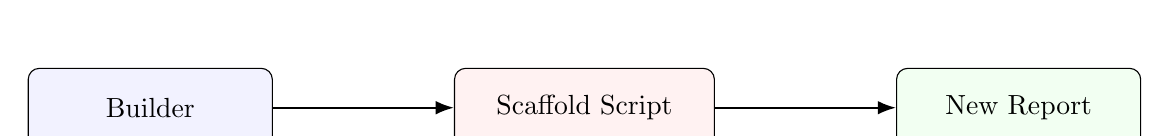
\begin{tikzpicture}[node distance=2.3cm, >=Latex]
    \node[draw, rounded corners, fill=blue!5, minimum width=3.1cm, minimum height=1cm] (template) {Builder};
    \node[draw, rounded corners, fill=red!5, right=of template, minimum width=3.3cm, minimum height=1cm] (generator) {Scaffold Script};
    \node[draw, rounded corners, fill=green!5, right=of generator, minimum width=3.1cm, minimum height=1cm] (project) {New Report};
    \draw[->, thick] (template) -- (generator);
    \draw[->, thick] (generator) -- (project);
  \end{tikzpicture}
  \caption{Flow from reusable builder to generated LaTeX project. \textit{Source: Compiled by the author.}}
  \label{fig:scaffold-flow}
\end{figure}

\section{Project Scope}
\label{sec:project-scope}

This scaffold standardizes project initialization while leaving the report content fully editable.

\subsection{Requirements}
\label{subsec:requirements}

\begin{itemize}
  \item The front matter includes a Table of Contents, List of Figures, and List of Tables.
  \item Bibliography management matches the analyzed project through \texttt{biblatex} with \texttt{biber}.
  \item The source tree remains chapter-oriented and uses \texttt{\textbackslash input} and \texttt{\textbackslash include}.
  \item Compilation is reproducible through a local Makefile and \texttt{latexmk}.
\end{itemize}

\section{Methodology and Rigor}
\label{sec:methodology-and-rigor}

\begin{tcolorbox}[colback=blue!3, colframe=upcblue, title=Validation checklist]
The generated project should compile with \texttt{make pdf} inside the project directory. A successful build confirms that the TOC, LOF, LOT, theorem list, and bibliography passes are wired correctly.
\end{tcolorbox}


%% ============================================================
%%  chap:project-planning.tex
%% ============================================================
\chapter{Project Planning}
\label{chap:project-planning}

\section{Description of Tasks}
\label{sec:description-of-tasks}

The builder decomposes the report into independently editable chapter files so the writing process stays modular as the project grows.

\section{Estimates and the Gantt Chart}
\label{sec:estimates-and-the-gantt-chart}

\begin{table}[H]
  \centering
  \begin{tabular}{@{}lcc@{}}
    \toprule
    Task & Estimated Hours & Output \\
    \midrule
    Analyze reference structure & 4 & Formatting notes \\
    Create LaTeX scaffold & 6 & Reusable project template \\
    Validate build chain & 2 & Working PDF generation \\
    \bottomrule
  \end{tabular}
  \caption{Illustrative task summary. \textit{Source: Compiled by the author.}}
  \label{tab:task-summary}
\end{table}

\begin{landscape}
\begin{figure}[p]
  \centering
  \begin{ganttchart}[
    x unit=0.7cm,
    y unit chart=0.8cm,
    vgrid,
    hgrid,
    title height=1,
    bar/.style={fill=upcblue!60},
    title/.style={fill=upcblue!10}
  ]{1}{6}
    \gantttitle{Illustrative Work Plan}{6} \\
    \gantttitlelist{1,...,6}{1} \\
    \ganttbar{Structure analysis}{1}{2} \\
    \ganttbar{Project scaffolding}{3}{5} \\
    \ganttbar{Compilation validation}{6}{6}
  \end{ganttchart}
  \caption{Illustrative Gantt chart included to preserve the same planning-oriented package stack as the reference report. \textit{Source: Compiled by the author.}}
  \label{fig:gantt-chart}
\end{figure}
\end{landscape}

\section{Risk Management, Alternative Plans, and Obstacles}
\label{sec:risk-management-alternative-plans-and-obstacles}

\begin{tcolorbox}[colback=red!3, colframe=fibred, title=Representative risks]
\begin{itemize}
  \item Missing LaTeX dependencies in the local TeX distribution.
  \item Manual edits that break the generated chapter include paths.
  \item Divergence between figure locations and \texttt{\textbackslash graphicspath}.
\end{itemize}
\end{tcolorbox}


%% ============================================================
%%  chap:budget-sustainability.tex
%% ============================================================
\chapter{Budget and Sustainability}
\label{chap:budget-sustainability}

\section{Budget}
\label{sec:budget}

\begin{table}[H]
  \centering
  \begin{tabular}{@{}lrr@{}}
    \toprule
    Item & Units & Cost \\
    \midrule
    Structural design time & 10 h & 300.00 \euro \\
    Build automation time & 3 h & 90.00 \euro \\
    Validation & 2 h & 60.00 \euro \\
    \midrule
    Total & 15 h & 450.00 \euro \\
    \bottomrule
  \end{tabular}
  \caption{Illustrative budget table in the same report style. \textit{Source: Compiled by the author.}}
  \label{tab:budget-summary}
\end{table}

\section{Sustainability}
\label{sec:sustainability}

Consistent project initialization reduces formatting churn, lowers maintenance overhead across reports, and improves readability for supervisors and evaluators\cite{pmbok_guide}.


%\chapter{Design}
\label{chap:design}

\section{Architecture}
\label{sec:architecture}

Use this chapter for the formal system or methodology design.

%\chapter{Implementation}
\label{chap:implementation}

\section{Implementation Details}
\label{sec:impldetails}

Use this chapter for implementation details and reproducibility notes.

%\chapter{Testing and Validation}
\label{chap:testing}

\section{Evaluation}
\label{sec:evaluation}

Use this chapter for experiments, validation, and testing results.

%\chapter{Conclusions}
\label{chap:conclusions}

\section{Conclusions}
\label{sec:conclusions}

Use this chapter for conclusions and future work.


\printbibliography[heading=bibintoc]

\end{document}
